\section {What you've got}

In the box you'll have a WebBrick 6.5 and any other peripherals that you've ordered.

\begin{figure}[H]
\centering
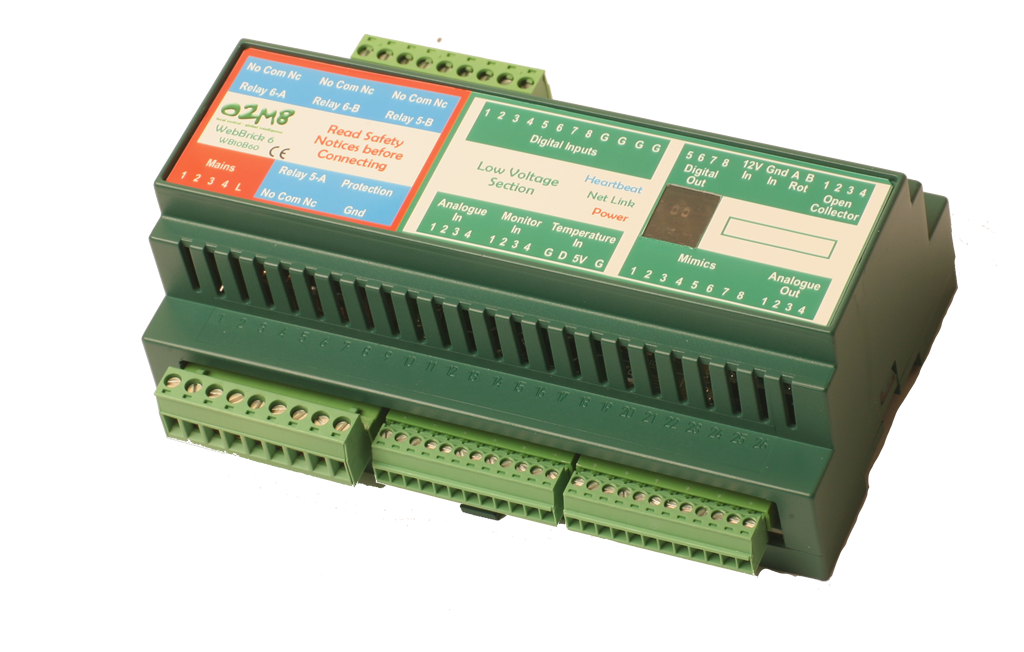
\includegraphics[width=0.6\textwidth]{PackShots/ObliquePackShot-WithoutCoin.png}
\end{figure}

Documentation can be accessed on http:://docs.webbrick.co.uk, utilities and additional software libraries can
be accessed from http://community.webbricksystems.com.

Usefull items are:
WebBrick monitor application for Windows (WebBrickMon), 
Python interpreter for Linux and Windows, 
Python library and example code and some PHP sample code. The PHP code is proof of concept 
stuff as Python is our preferred environment and our active environment.

\section{Overview}

What is a WebBrick? It is a network connected control and automation product designed around the principle 
of 'local control - global intelligence'. This means that most of the time control is handled locally, but a 
system as a whole can be made more intelligent through the use of some central control
(for example the Webbrick Gateway) that provides the global intelligence. 
i.e. Lights for a room are a local issue, but heating is 
more of an overall control issue. This also means that you are
not dependant on a single control system for the complete system, you can always switch on the lights 
in this room while someone is making changes to a global control system.

Control can be done through a WebBrick's web interface, through its physical inputs or using remote commands.

\section{Connections}

\subsection{Outputs}

The webbrick has the following types of outputs.

\begin{tabular}{l|p{12cm}}
Digital&These are used to connect to simple on off devices that can be switched on by a low voltage, i.e. LED
lighting.\\

Open collector&These are used to connect to relays and similar devices that need the input connecting to 
ground to switch on.\\

Mains Triacs.&These these enable mains voltage devices to be switched 
on and off by the webbrick directly and are driven by 4 of the digitl outputs.\\

Relay&These are double pole changeover relays that are driven by 2 of the digital outputs.
A changeover contact connects 1 connection to one of 2 other connections, each relay has two changeover
contacts. These are intended for use by devices such as curtains which need connections swapping over\\

Analogue&These provide a 0 to 10V voltage which can be connected to lighting dimmers or any thing that uses
a variable voltage to control it.\\

Mimics&These are pulse width modulated (PWM) digital outputs intended to connect to LED status indicators, the use 
of PWM allows the LED brightness to be adjusted. They
can be configured to show the state of a digital or analogue output channel or directly controlled
over the network connection. When the output level is changed they fade over a short period of time to the
new level.\\

Infra red transmitter&This can be connected to the WebBrick and then the WebBrick programmed to send RC5
encoded commands to devices that can understand this infra red dialect.\\
\end{tabular}

\subsection{Inputs}

The webbrick has the following types of inputs.


\begin{tabular}{l|p{12cm}}
Digital&These are designed primarily for switches but can be used to connect input devices that only have 
two states, see reference manula for details on this.\\

Analogue&Theseare used to connect input devices that provide a vraiable voltage, i.e. rotary controls or
humidity sensors. See reference manula for voltage levels.\\

Temperature&This is used to connect up to 5 temperature sensors, they share the 3 wires going 
from 1 sensor to the next.\\

Rotary Encoder&This is used to connect a continuously rotating knob to a webbrick to adjust the 
first analogue output.\\

Infra red receiver&Can be connected to the WebBrick and then the WebBrick programmed map some 
received RC5 dialect commands to be the equivalent of digital inputs. All RC5 commands received
commands are sent over the network connection and can then be handled within the central controller.\\
\end{tabular}

\section{Getting Started}

First you need to connect 12V power to the WebBrick, and then provide a network connection.

\begin{figure}[H]
\centering
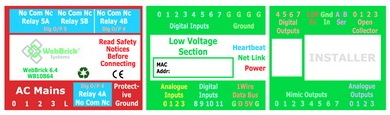
\includegraphics[width=0.7\textwidth]{Images/TopCover.jpg}
\end{figure}

\begin{tabular}{l|p{12cm}}
Top left&Most Relay Contacts\\
Bottom left&Mains and remaining Relay Contacts\\
Center top&Digital inputs\\
Center bottom&Analogue inputs, temperaure\\
Right top&power, digital outputs\\
Right bottom&Status Indicators and analogue outputs\\
\end{tabular}

\subsection{Power}

Power is connected to the connector on the top right hand side of the case when you look at the top with
the writing on the label facing you and the right way up, the larger connectors will be on your left hand side.
The supply needs to be 12V-15V DC and it should be regulated. The polarity is important; the plus rail should be connected as 
indicated on the overlay on top of the case. 
To prevent injury the mains connections and relay connections are through physically larger connectors, 
these are on the left hand side of the case. (Disconnect any mains supply when working on the webbrick connectors).
The correct pins for the power supply input are pins 7 and 8 on the top right connector with PIN 8 being +12V 
and PIN 7 being the 0v line
from the power supply. NOTE pin1 is on the outer top edge of the case, so count right to left.

When you power up the WebBrick, the following should happen:

\begin{tabular}{l|l|p{12cm}}
LED name&Colour&description\\
\hline
Power&red&This should light immediately\\
Network&green&Lights for 0.25 seconds then waits for network link(stays lit if network is connected and available)\\
Heart Beat&blue&You'll see this flash rapidly during start-up then settle to 1Hz.
	Once at 1Hz the WebBrick has booted and is ready to use\\
\end{tabular}

If the webbrick fails to power up, check the power connections are the correct way round, there is a polarity
protection diode to prevent damage if incorrectly connected.

\subsection{Network}

Take an Ethernet cable from your network hub and plug into the RJ45 connector on the top right of the unit,
above the power connector, the locking tab is downwards intentionally so as to require a small screwdriver 
to release it.

When you plug the cable in the Green LED should come on to indicate a network connection has been found.

\section{Setting IP address}

The WebBrick default IP address is 10.100.100.100 with a 255.0.0.0 subnet mask, DHCP is not enabled. 
If your network is not on 10.0.0.0 then you can use WebBrickMon to set the address to something valid 
on your network or you can give a computer an additional IP address.

%TODO need to add details about identifying an IP address to use.

\subsection{Using WebBrickMon}
Download webbrickmon from community.webbricksystems.com.
Its primary purpose is to find 
unconfigured WebBricks on your network and optionally set the IP address they are using, it can 
be used to see what UDP events are coming out of the WebBrick.

When you start it for the first time, Windows may generate a warning about the application opening a network port, which of course it needs to.  
Unblock the application and you'll see a display like:
\begin{figure}[H]
\centering
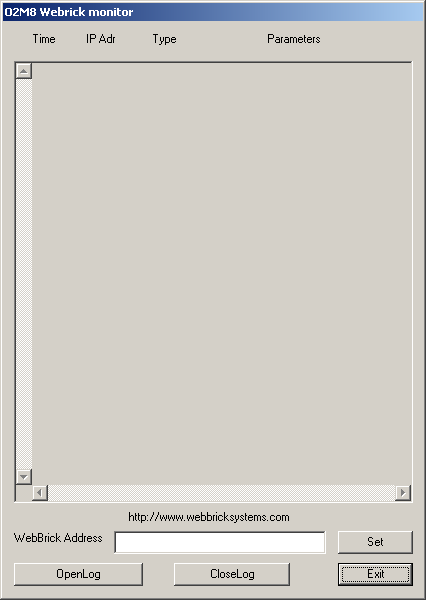
\includegraphics[width=0.6\textwidth]{Images/WebBrickMon.png}
\end{figure}

You should be seeing NewNode events and possibly some others. To set IP address enter a suitable value 
in dotted form i.e. "192.168.1.1" in the dialog at the bottom and then click on SET. The monitor will 
now wait for a WebBrick to send either New Node or an Alert packet and then 
send the new IP address to the WebBrick. You will then see events coming from the new IP address.

The main part of the monitor dialog shows WebBrick events with some decoding. First column is time, 
followed by source IP address and 
a sequence number. Then follows Event type and Event code, a text translation of the event code.


\subsection{Adding IP address to a windows computer}
There is no need to overwrite any of your existing network configuration in Windows.  
Under the TCP/IP advanced configuration tab
use add address to give you a dialog like:

\begin{figure}[H]
\centering
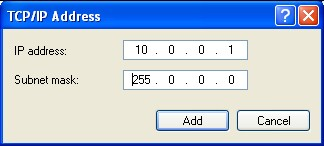
\includegraphics[width=0.6\textwidth]{Images/addIP.jpg}
\end{figure}

To locate the above go to Start/Setting/Network Connections or Control Panel Network connections and select the 
Local Area Connection. Select Properties and scroll down to find TCP/IP and click properties again. Then Advanced button.

\section{Factory Reset switch}
There is a button that resets the WebBrick to its factory default, if it is pushed at power up then the configuration is erased and then set 
to factory default values. If the factory reset button is pushed after power up the WebBrick will send Alert events (event code AA) 
for 60 seconds, this is an assistance to locate a WebBrick IP address if unknown. To access the button use a credit card or similar 
and insert flat between the case and the connector that is under the Ethernet connection, its location is intentional to reduce 
finger trouble.

Note if the IP address has been set for you at manufacture then the IP address will not be modified by a factory
reset.

\section{Browsing to your WebBrick}

Having completed one of the two steps in "Setting IP address" you should now be able to access the WebBrick own webserver
by entering either 10.100.100.100 into your browser (Internet Explorer or Firefox) or the address you entered in WebBrickMon.

You should see a page which looks like:

\begin{figure}[H]
\centering
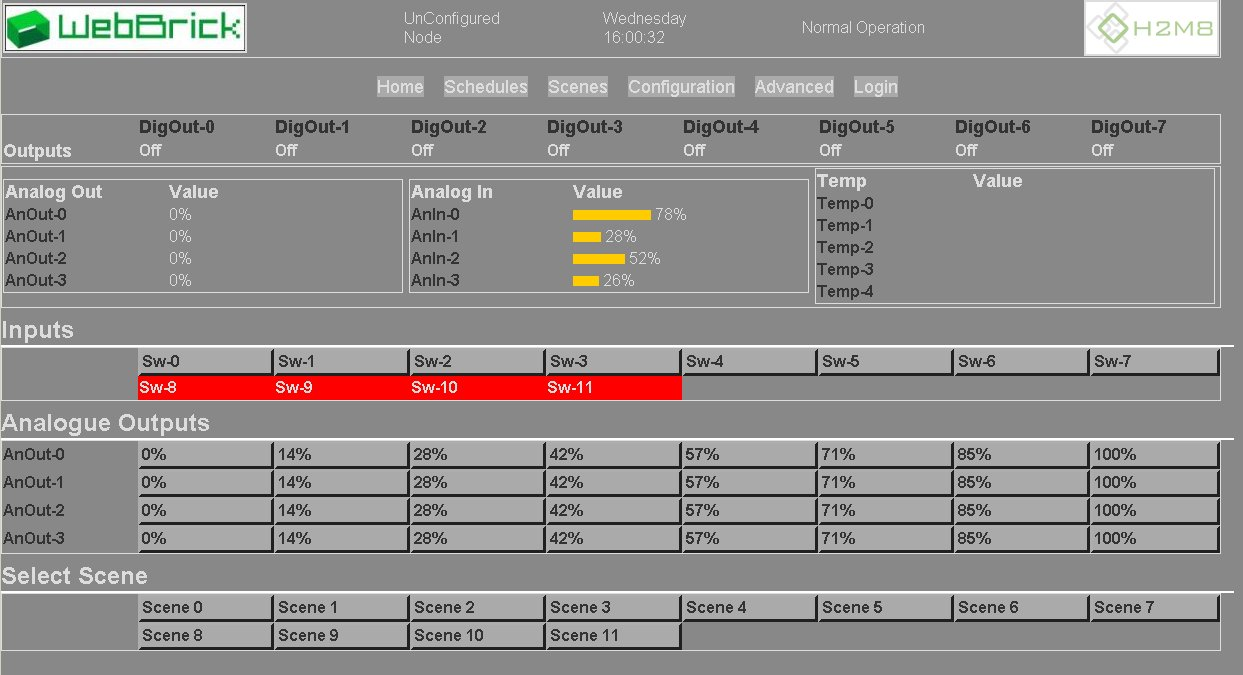
\includegraphics[width=1.0\textwidth]{Images/uncHome.jpg}
\end{figure}

This shows that the WebBrick is a new node and that there is no temperature sensors attached.  

\section{Home page}
The WebBrick home page has control buttons that can be used to act on WebBrick outputs, by
default these are enabled. If you set a user password (See manual) then these will be disabled until
you login. This screen is split into:

\begin{tabular}{l|p{12cm}}
i)&a section showing state a of digital outputs.\\
ii)&a section showing state a of analogue outputs.\\
iii)&a section showing state a of analogue inputs.\\
iv)&a section showing state a of temperature sensors.\\
v)&a set of buttons that can be used to simulate a button press on the digital inputs, these then perform 
what ever is configured for that input.\\
vi)&a set of buttons that adjust the analogue outputs to one of the set points.\\
vii)&a set of buttons that initiate one of the scenes, there are no scenes configured by default so they will
do nothing.\\
\end{tabular}

\section{Toggling an output channel}

Digital output channels 5 and 6 are connected to a pair of change over relays (DPDT relays).  If you operate those channels you should hear the relays
click.  To do this go to the WebBrick home page.  Look for the section called 'Controls' and click on the Sw-5 and Sw-6 buttons.  You'll hear the relays
operate and the resulting page should look like:

\begin{figure}[H]
\centering
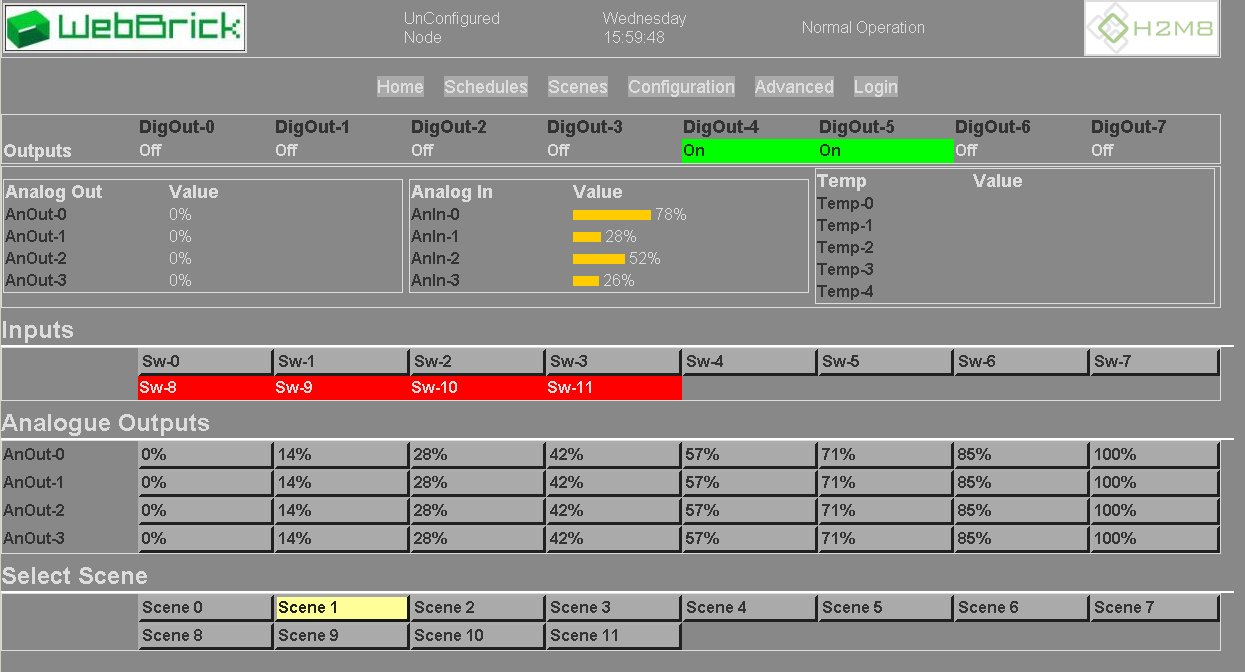
\includegraphics[width=0.9\textwidth]{Images/homeRelays.jpg}
\end{figure}

Note that the DigOut-4 and DigOut-5 fields in the output section are now green.  This indicates that these digital outputs are on.  Also note that the Sw-6 button 
is highlighted in pale yellow.  This is because the mouse was left over the button during the screenshot.  The point of the pale yellow mouse over is to 
let you know that you can click on something.

If you go to the configuration page and find that nothing has a mouse over its because you are not logged in.  Login will time out after 5 minutes, this is 
because for home page operations you need not be logged in, but for configuration operations you need to be logged in.

\section{Temperaure sensors}

If we connect a temperature sensor to the WebBrick, read the datasheet that came with your temperature sensor for connection
details (power off the WebBrick for this operation).
Wwe should have a page which looks like:

\begin{figure}[H]
\centering
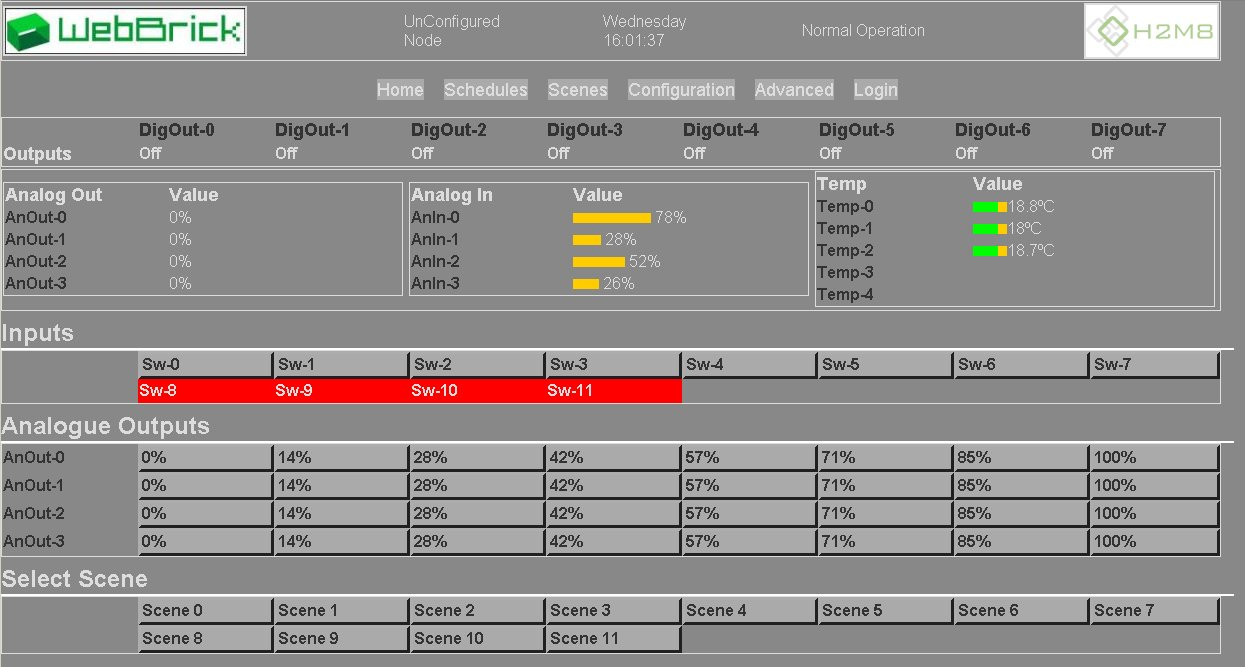
\includegraphics[width=0.9\textwidth]{Images/sensHome.jpg}
\end{figure}

This shows that the temperature sensor is working, in this case three sensors are connected. 
Now we can login to the WebBrick to set some simple parameters.

\section{Basic Configuration}

Click the login link to get a page which looks like:

\begin{figure}[H]
\centering
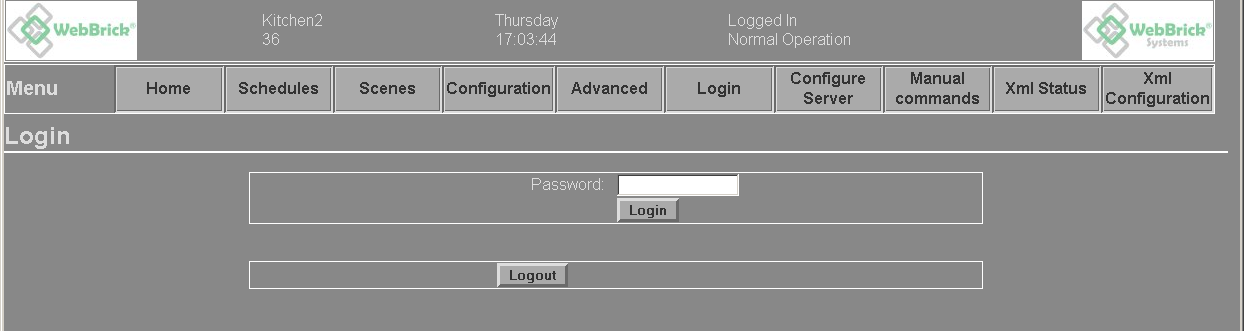
\includegraphics[width=0.8\textwidth]{Images/login.jpg}
\end{figure}
The default 
configuration password is "password". 
Be sure to click the login button.  If your login was sucessful, you will be taken to:

\begin{figure}[H]
\centering
\includegraphics[width=0.8\textwidth]{Images/configuration.jpg}
\caption{WebBrick Configuration Home Page}
\end{figure}

The banner section at the top will indicate LoggedIn, from there you can go click the 
configure server link to get a page like this:

\begin{figure}[H]
\centering
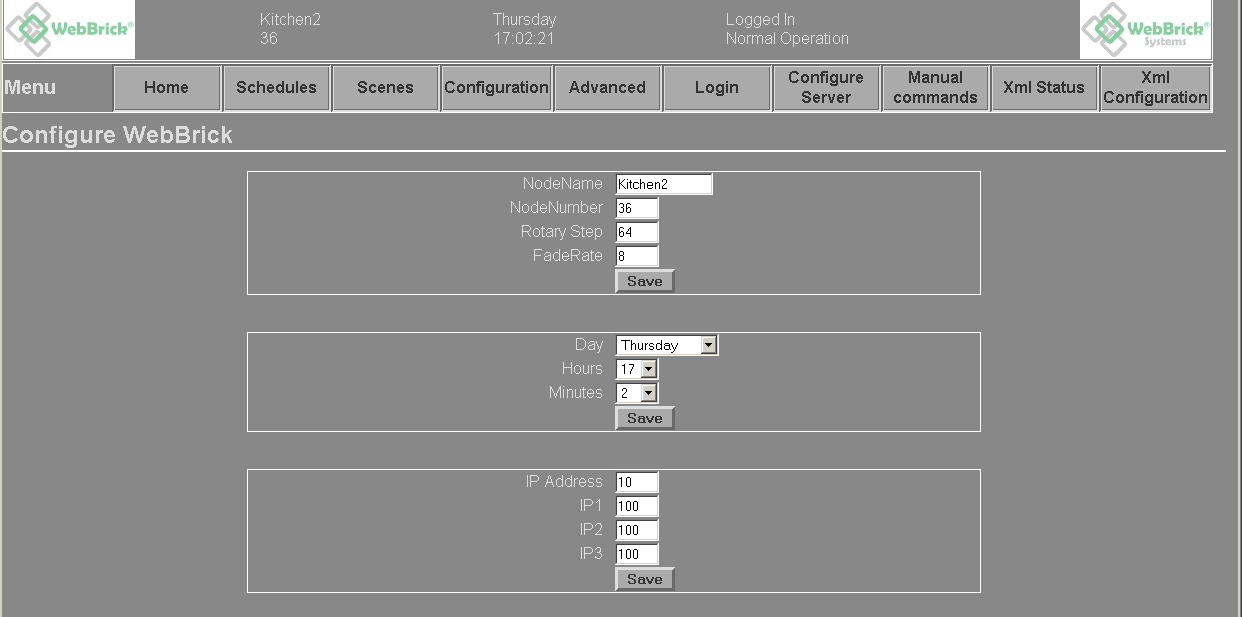
\includegraphics[width=0.9\textwidth]{Images/ConfigureServer.jpg}
\end{figure}

You should at least enter the node name and number (the number should be between 1 and 254) you click 
the first save button. You can also set the onboard clock if neccessary.

Some of the configuration elements are straightforward, however others mean that you'll 
really need to have a look at the full manual.

\section{A simple configuration}

In this configuration we will show how an output channel can be switched on above 28 deg C and switched off again at 24 deg C.

First check that you are logged in to your WebBrick, then select the configuration page. 
From here, look at the temperature sensors section, for each sensor there are two lines
the first specifies a low threshold and its trigger action, the second a high threshold and its trigger action:

\begin{figure}[H]
\centering
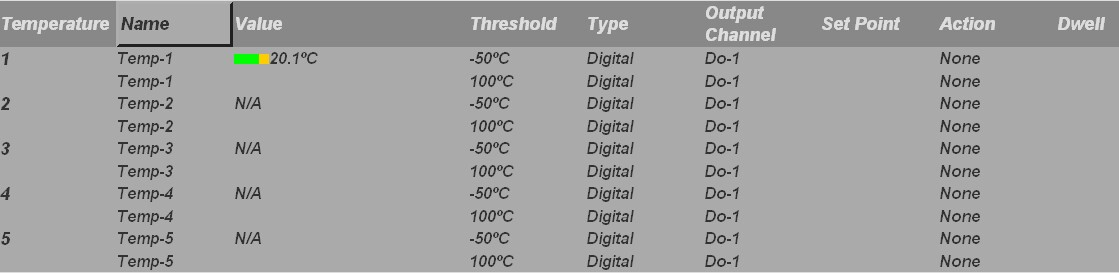
\includegraphics[width=0.9\textwidth]{Images/tempCfg.jpg}
\end{figure}

Now click on the first section, you'll get a configuration dialog like:

\begin{figure}[H]
\centering
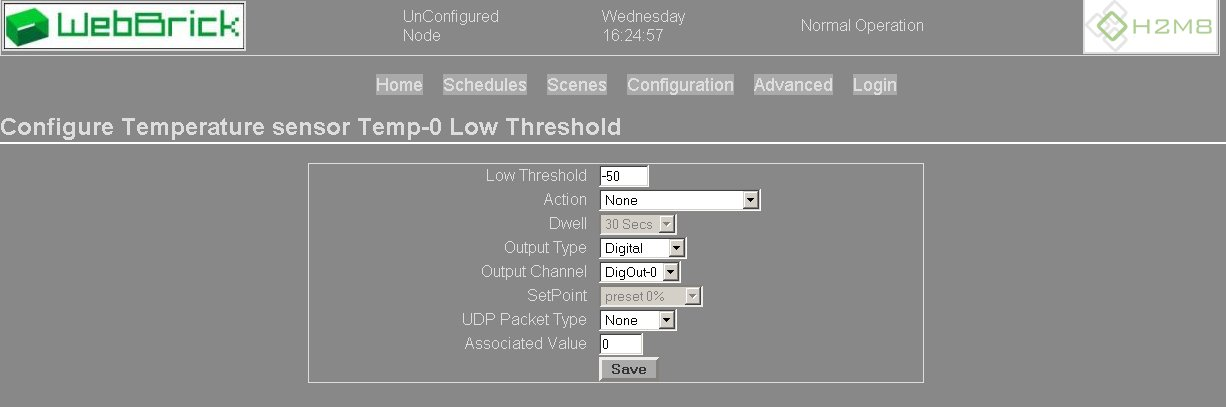
\includegraphics[width=0.6\textwidth]{Images/tempLowCfg.jpg}
\end{figure}

Now enter the value '24' in the first entry, this is the threshold value,
Select Off as the action type from the action drop down box,
Select Digital from the output type drop down box,
Select 'DigOut-0' from the output drop down box,
Leave UDP Type and assocaited value as is.
And then click on Save button. This process is the process confuguring a trigger and is common across
all the inputs in that all inputs can target an trigger action to all possible outputs. The dwell drop 
down boxes will be greyed out unless you select a Dwell or Dwell Cancel action. Similarly the SetPoint drop down
will be greyed out unless you select an Analogue channel as the output type.

Do the same thing for the high threshold but enter 28 as the threshold value.

\begin{figure}[H]
\centering
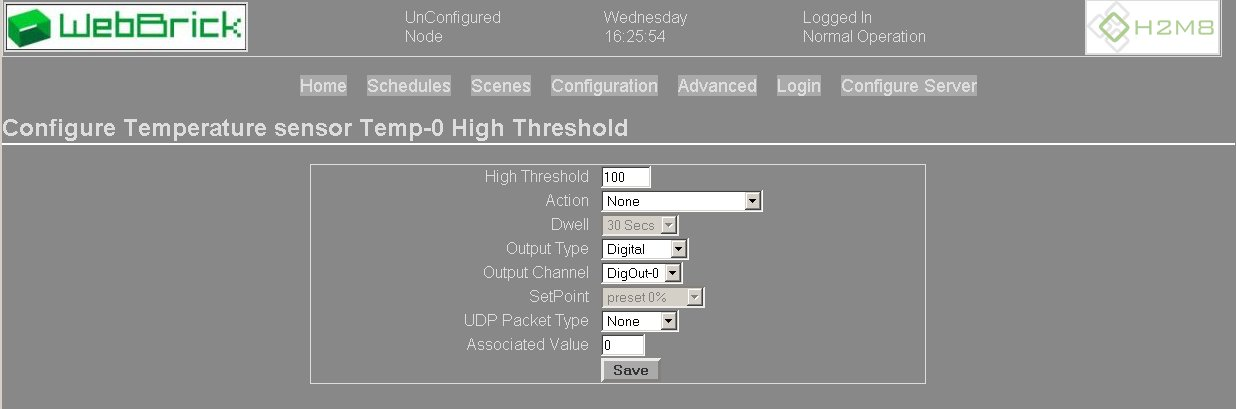
\includegraphics[width=0.6\textwidth]{Images/tempHighCfg.jpg}
\end{figure}

Now hold the temperature sensor between your fingers and refresh the home page to watch the temperature rising.  
See that digital output 'DigOut-1' goes to the ON state
above 28 deg C.  Now let go of the sensor and watch the temperature drop.  
See that 'DigOut-1' goes OFF below 24 deg C.

If you target the trigger at DigOut-4 or DigOut-5 you will hear the relays toggle.

\section{Quick tour of WebBrick and XML}

In order to drive standards based automation, the WebBrick can deliver both status and configuration information using XML.  
To view the XML source, go to the advanced page.  Here you'll find the links to view the XML status and XML configuration. 
You need not be logged in to see these. The content of these is documented in the mainreference manual and the python
code on the communtiy site has some helpers which will retrieve the XML from a WebBrick and extract data which can then be used 
to make decisions. 

\section{WebBrickMon}

You have already met WebBrickMon briefly in using it to set IP addresses, in a small WebBrick network it can be
used to provide some debugging information for those who are building extended controls from server and want to
see what�s happening. it has no filtering so if you have a network with a large number of 
WebBrick on it you may find it hard to see the data.

WebBrick send events using UDP and these are what WebBrickMon listens for. For each event it receives it prints some
output identifying the WebBrick it came from and the channel type and number that it refers to. Depending on the channel 
type it will list some additional data, see the WebBrick manual for the content of UDP events.

\section{Technical Support}
We prefer technical support questions to be sent by email and we aim to respond in 1 working day, please address support questions to
technical@webbricksystems.com or visit http://community.WebbrickSystems.com

